\documentclass[letterpaper,spanish,reprint,nofootinbib,showkeys,aps]{revtex4-2}

%%%%%%%%%%%%%%%%%%%%%%%%%%%%%%%%%%%%%%%%%%%%%%%%%%%%%%%%%%%%%%%%%%%%%%%%%%%%
% PAQUETES USUALES
\usepackage[T1]{fontenc}
\usepackage[utf8]{inputenc}
\usepackage[spanish]{babel} 
\usepackage{calc}
\usepackage{amsmath,bm,amssymb}
\usepackage{fancyhdr}
\usepackage{pythonhighlight}
\usepackage{graphicx}
\usepackage{float}\usepackage{xcolor}
%para escribir código%%%%%%%%%%%%%%
\usepackage{algorithm}
\usepackage{algpseudocode}
\usepackage{listings}
\usepackage{color, xcolor}
%%%Algunos comandos útiles para el PDF generado%%%
\usepackage[unicode=true,pdfusetitle, bookmarks=true,bookmarksnumbered=false,bookmarksopen=false, breaklinks=false,pdfborder={0 0 1},backref=false,colorlinks=true] {hyperref}
\hypersetup{
 citecolor=dkgreen,linkcolor=blue,urlcolor=blue}
%%% PARA TEOREMAS NUEVOS
\usepackage{amsthm}
\renewcommand{\qedsymbol}{\tiny{$\blacksquare$}}
\newenvironment{solucion}{\begin{proof}[\textcolor{magenta}{Solución}]}{\end{proof}}
\usepackage{mdframed}
\usepackage[many]{tcolorbox}
\usepackage{thmtools}


%%%%%%%%%%%%%%%%%%%%%%%%%%%%%%%%%%%%%%%%%%%%%%%%%%%%%%%%%%%%%%%%%%%%%%%%%%%%
%%%%%%%%%%%%%%%%%%%%%%%%%%%%%%%%%%%%%%%%%%%%%%%%%%%%%%%%%%%%%%%%%%%%%%%%%%%%
%%%%%%%%%%%%%%%%%%%%%%%%%%%% MARGENES %%%%%%%%%%%%%%%%%%%%%%%%%%%%%%%%%%%%%%
%%%%%%%%%%%%%%%%%%%%%%%%%%%%%%%%%%%%%%%%%%%%%%%%%%%%%%%%%%%%%%%%%%%%%%%%%%%%
%%%%%%%%%%%%%%%%%%%%%%%%%%%%%%%%%%%%%%%%%%%%%%%%%%%%%%%%%%%%%%%%%%%%%%%%%%%%

\parskip=5pt
\hoffset = 0pt
\headsep = 0.8 cm % estaba en 1.5 cm, lo cambie para el header de la imagen
\setlength{\parindent}{0cm}

%%%%%%%%%%%%%%%%%%%%%%%%%%%%%%%%%%%%%%%%%%%%%%%%%%%%%%%%%%%%%%%%%%%%%%%%%%%%
%%%%%%%%%%%%%%%%%%%%%%%%%%%%%%%%%%%%%%%%%%%%%%%%%%%%%%%%%%%%%%%%%%%%%%%%%%%%
%%%%%%%%%%%%%%%%%%%%%%%%% EJERRCICIOS  %%%%%%%%%%%%%%%%%%%%%%%%%%%%%%%%%%%%%
%%%%%%%%%%%%%%%%%%%%%%%%%%%%%%%%%%%%%%%%%%%%%%%%%%%%%%%%%%%%%%%%%%%%%%%%%%%%
%%%%%%%%%%%%%%%%%%%%%%%%%%%%%%%%%%%%%%%%%%%%%%%%%%%%%%%%%%%%%%%%%%%%%%%%%%%%

\newtcolorbox[auto counter,number within=section]{ejercicio}[1][]{
% ESTO ES PARA LA CAJA GENERAL
breakable, % por si cambias de pagina
enhanced, % estilo general
% TITULO MODIFICACIONES
coltitle= black,
colbacktitle= white,
titlerule= 0mm,
colframe = magenta,
fonttitle=\bfseries,
title= Ejercicio~\thetcbcounter,
% CAJA LINEA MODIFICACIONES
boxed title style={
  sharp corners,
  rounded corners=northwest,
  rounded corners=northeast,
  % outer arc=0pt,
  % arc=0pt,
  },
% CONTENIDO MODIFICACIONES
colback = white,
fontupper = \itshape,
coltext =  black,
% MARCO MODIFICACIONES
rightrule=0mm,
toprule=0pt,
bottomrule= 0pt,
leftrule = 4pt
}

%%%%%%%%%%%%%%%%%%%%%%%%%%%%%%%%%%%%%%%%%%%%%%%%%%%%%%%%%%%%%%%%%%%%%%%%%%%%
%%%%%%%%%%%%%%%%%%%%%%%%%%%%%%%%%%%%%%%%%%%%%%%%%%%%%%%%%%%%%%%%%%%%%%%%%%%%
%%%%%%%%%%%%%%%%%%%%%%%%% MEMO PYTHON Y C %%%%%%%%%%%%%%%%%%%%%%%%%%%%%%%%%%
%%%%%%%%%%%%%%%%%%%%%%%%%%%%%%%%%%%%%%%%%%%%%%%%%%%%%%%%%%%%%%%%%%%%%%%%%%%%
%%%%%%%%%%%%%%%%%%%%%%%%%%%%%%%%%%%%%%%%%%%%%%%%%%%%%%%%%%%%%%%%%%%%%%%%%%%%


\definecolor{dkgreen}{rgb}{0.9,0.6,0.8}
\definecolor{blue}{rgb}{0.0,0.49,0.4}
\definecolor{gray97}{gray}{.97}
\definecolor{gray75}{gray}{.75}
\definecolor{gray45}{gray}{.45}
\definecolor{codegreen}{rgb}{0,0.6,0}
\definecolor{codegray}{rgb}{0.5,0.5,0.5}
\definecolor{codepurple}{rgb}{0.58,0,0.82}
\definecolor{backcolour}{rgb}{0.95,0.95,0.92}

\lstdefinestyle{mystyle}{
    backgroundcolor=\color{gray97},
    commentstyle=\color{cyan!75!black},
    keywordstyle=\color{magenta},
    numberstyle=\tiny\color{codegray},
    stringstyle=\color{codepurple},
    basicstyle=\ttfamily\footnotesize,
    breakatwhitespace=false,
    breaklines= true,
    captionpos=b,
    keepspaces=true,
    numbers=left,
    numbersep=5pt,
    showspaces=false,
    showstringspaces=false,
    showtabs=false,
    tabsize=2,
    language=bash,   %% PHP, C, Java, etc... bash is the standard
    extendedchars=true,
    inputencoding=latin1
}

\lstset{style=mystyle, literate =
                        {í}{{\'i}}1
                        {á}{{\'a}}1
                        {é}{{\'e}}1
                        {ó}{{\'o}}1
                        {ú}{{\'u}}1
                        {ñ}{{\~n}}1
                        {ü}{{\"u}}1
                            }

%%%%%%%%%%%%%%%%%%%%%%%%%%%%%%%%%%%%%%%%%%%%%%%%%%%%%%%%%%%%%%%%%%%%%%%%%%%%
%%%%%%%%%%%%%%%%%%%%%%%%%%%%%%%%%%%%%%%%%%%%%%%%%%%%%%%%%%%%%%%%%%%%%%%%%%%%
%%%%%%%%%%%%%%%%%%%%% ##ENCABEZADOS Y NUMERACION %%%%%%%%%%%%%%%%%%%%%%%%%%%%%
%%%%%%%%%%%%%%%%%%%%%%%%%%%%%%%%%%%%%%%%%%%%%%%%%%%%%%%%%%%%%%%%%%%%%%%%%%%%
%%%%%%%%%%%%%%%%%%%%%%%%%%%%%%%%%%%%%%%%%%%%%%%%%%%%%%%%%%%%%%%%%%%%%%%%%%%%

\pagestyle{fancy}
\fancyhf{}
\fancyfoot{\thepage}
\fancyfoot[R]{\small{\textsc{Sarahi García, Ramón Ruíz}}}
\fancyfoot[L]{\small{\textsc{Reconocimiento estadístico de patrones}}}
\chead{\includegraphics[scale=.27]{/Users/ely/Documents/Plantilla/Figures/waves.pdf}}
\renewcommand{\headrulewidth}{0pt}
\renewcommand{\footrulewidth}{0pt}

%%%%%%%%%%%%%%%%%%%%%%%%%%%%%%%%%%%%%%%%%%%%%%%%%%%%%%%%%%%%%%%%%%%%%%%%%%%%
%%%%%%%%%%%%%%%%%%%%%%%%%%%%%%%%%%%%%%%%%%%%%%%%%%%%%%%%%%%%%%%%%%%%%%%%%%%%
%%%%%%%%%%%%%%%%%%%%%%%%%%%%%%%%%%%%%%%%%%%%%%%%%%%%%%%%%%%%%%%%%%%%%%%%%%%%
%%%%%%%%%%%%%%%%%%%%%%%%%%%%%%%%%%%%%%%%%%%%%%%%%%%%%%%%%%%%%%%%%%%%%%%%%%%%

%%%Declaración de operadores%%%
\DeclareMathOperator{\sech}{sech}

%%%%%%%%%%%%%%%%%%%%%%%%%%%%%%%%%%%%%%%%%%%%%%%%%%%%%%%%%%%%%%%%%%%%%%%%%%%%
%%%%%%%%%%%%%%%%%%%%%%%%%%%%%%%%%%%%%%%%%%%%%%%%%%%%%%%%%%%%%%%%%%%%%%%%%%%%
%%%%%%%%%%%%%%%%%%%%%%%%%%%%%%%%%%%%%%%%%%%%%%%%%%%%%%%%%%%%%%%%%%%%%%%%%%%%
%%%%%%%%%%%%%%%%%%%%%%%%%%%%%%%%%%%%%%%%%%%%%%%%%%%%%%%%%%%%%%%%%%%%%%%%%%%%

\begin{document}

\preprint{Reconocimiento estadístico de patrones}
\title{\Large{\textbf{Estudio de INP en México}}}
%\thanks{A footnote to the article title}
\author{Sarahi García, Ramón Ruíz}
\email{yesenia.garcia@cimat.mx, ramon.ruiz@cimat.mx}
\affiliation{\vspace{0.15cm}Centro de Investigación en Matemáticas CIMAT}
\thanks{REP, a  cargo de Dr. Johan Van horebeek}


%%%%%%%%%%%%%%%%%%%%%%%%%%%%%%%%%%%%%%%%%%%%%%%%%%%%%%%%%%%%%%%%%%%%%%%%%%%%
%%%%%%%%%%%%%%%%%%%%%%%%%%%%%%%%%%%%%%%%%%%%%%%%%%%%%#0Abstract%%%%%%%%%%%%%%%
%%%%%%%%%%%%%%%%%%%%%%%%%%%%%%%%%%%%%%%%%%%%%%%%%%%%%%%%%%%%%%%%%%%%%%%%%%%%
%%%%%%%%%%%%%%%%%%%%%%%%%%%%%%%%%%%%%%%%%%%%%%%%%%%%%%%%%%%%%%%%%%%%%%%%%%%%

\begin{abstract}
\begin{center}
\small{11 de Diciembre de 2023}
\end{center}
\vspace{0.6cm}


\end{abstract}

\maketitle

%%%%%%%%%%%%%%%%%%%%%%%%%%%%%%%%%%%%%%%%%%%%%%%%%%%%%%%%%%%%%%%%%%%%%%%%%%%%
%%%%%%%%%%%%%%%%%%%%%%%%%%%%%%%%%%%%%%%%%%%%%%%%%%%#1INTRODUCION%%%%%%%%%%%%%
%%%%%%%%%%%%%%%%%%%%%%%%%%%%%%%%%%%%%%%%%%%%%%%%%%%%%%%%%%%%%%%%%%%%%%%%%%%%



\section{Preguntas de interes}

\begin{itemize}
\item ¿Cómo se relaciona la frecuencia de viajes de un usuario con su edad?
\item ¿El género tiene un efecto significativo en la duración y/o frecuencia de los viajes?
\end{itemize}

\section{Introducción}



El Índice Nacional de Precios al Consumidor (INPC) es un indicador de la evaluación y comprensión de la dinámica económica des país. Esta diseñado para estimar la evolución de los precios de los bienes y servicios consumidos por las familias de México.

Existe complejidad inherente a la medición de las variaciones de precios pues, entre otros factores, existe una amplia gama de artículos y servicios de consumo así como una constante fluctuación en los precios. Además, la asincronía en los cambios de precios y sus variaciones de velocidad agregan un nivel adicional de complejidad al análisis.

En este contexto, el presente se enfoca en analizar los precios de una amplia gama de productos en diversas ciudades de México. Utilizando datos muestrales, exploramos las fluctuaciones en los precios de nueve productos a lo largo del tiempo y en diferentes ubicaciones geográficas del país. Empleamos técnicas de análisis estadístico y visualización de datos, incluyendo dendrogramas y heatmaps, para identificar patrones y relaciones significativas en los datos.

La información recopilada para este análisis proviene de la base de datos proporcionada por una de las herramientas de del INPC del INEGI: \textbf{Consulta precios promedio}, que contiene registros de precios de distintas marcas y/o proovedores de una serie de productos y servicios en 55 ciudades que se consumen en todo el país. Las cotizaciones de los productos en esta base de datos son principalmente mensuales y se encuentran desde el mes de Agosto del año 2018.

Debido a la extensa cantidad de productos y servicios nos centraremos exclusivamente en los siguientes productos mostrados en \ref{base}, desde el mes de agosto de 2018 hasta el mes de marzo de 2024 de las 55 ciudades. Para un mejor manejo y representación visual de los datos se modificaron, y/o quitaron
algunas de las filas, de modo que para cada producto/servicio tenemos un único proveedor/marca. 



\begin{figure} [H]
	\begin{center}
		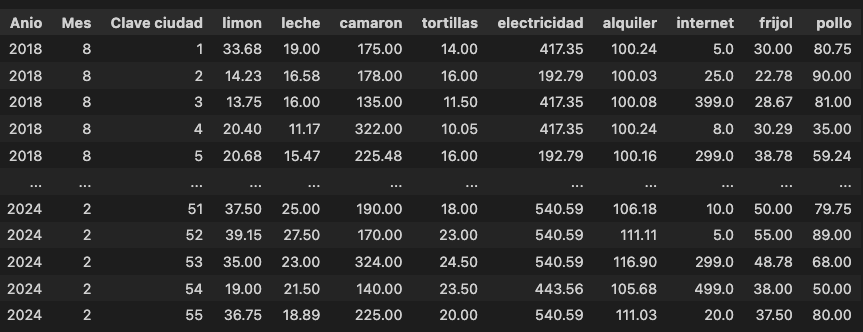
\includegraphics[scale=0.28]{/Users/ely/Documents/Maestria/segundo_semestre/cimat2023-1/patrones/Proyecto_1/imgenes/base.png}
		\caption{Datos utilizados para este trabajo}
		\label{base} 
   \end{center} 
\end{figure}




\section{Análisis Exploratorio }


\subsection*{Usuarios}
A continuación se presentan algunas de las carterísticas de los usurios de MiBici del conjunto de datos mencionado
hay \textbf{17282 distintos usuarios} que utlizaron, de los cuales 11668 son hombres y 5384 son mujeres {cantidadgenero}. 


Se puede apreciar en {edad} que la mayoría de los usuarios son adultos entre 25 y 40 años. La edad mínima
registrada es de 20 años y ls máxima de 106. 



Por otro lado, si hacemos la distinción de edades por género, como muestran los siguientes boxplots {edadygen}
podemos observar que en el género masculino el rando intercuantil abarca desde 30 hasta más de 40 años mientras que 
el de las mujeres inicia casi igual pero no alcanza los 40 años.




\subsection*{Viajes}
Algunas características que podemos obtener sobre los viajes a partir de los datos son los horarios y días de la semana 
más concurridos, la duración de los viajes y las estaciones más y menos utilizadas. A continuación daremos un panorama
general sobre los viajes que se realizan con MiBici.



De las gráficas {dia}, {hora} y {duracion} podemos observar que la cantidad de viajes disminuye significativaente
los fines de semana, la hora en que los usuarios más utilizan Mibici es las 18:00 y desde esa hora donde se alcanza el máximo,
el número de viajes decrece hasta su mínimo a las 23:00. Además la mayoría dura entre 6 y 14 minutos, en promedio, duran 11.





En la figura {dia}, la diferencia más relevante se aprecia entre el fin de semana y el resto de los dias, aunque sí se observa un crecimiento
de lunes a viernes.



Los máximos más relevantes de la figura {hora},se encuentran a las 8:00 y a las 18:00 y por la noche, después de las 20:00 se tiene concurrencia. No 
hay datos desde las 12:00 hasta ls 6:00.

%\begin{figure} [H]
%	\begin{center}
%		\includegraphics[scale=0.44]{/Users/sara/Documents/Maestria/primer_semestre/analisis/proyecto/analisis_exploratorio/viajes/duracion.png}
% 		\caption{Histograma de viajes por duración}
% 		\label{duracion} 
%    \end{center} 
%\end{figure}

En la primer gráfica de la figura {duracion}, se aprecia la distribución de duración de los viajes, sin embargo, debido a que hay algunos datos
que indican viajes de hasta 500 minutos, no se puede apreciar el lugar donde se encuentra la mayor concentración de datos,
por esta razón en la gráfica de abajo se realizó un zoom al intervalo [0,40], de esta manera puede observarse
mejor el histograma.
Hay un pico significante al inicio, lo que indica que una alta cantidad de viajes dura menos de uno o dos minutos. 


Podemos extraer un poco más de información si formamos un nuevo DataFrame donde
agruprmos los datos por usuario y agregamos una columna
que cuente el número de viajes de cada usuario que haya utilizado MiBici en Enero de 2019 y otra que indique 
el grupo de edad al que pertenece cada usuario (rangos=[20,25, 30,35, 40,45, 50,55, 60,65, 70,75, 80]).


%\begin{figure} [H]
%	\begin{center}
%		\includegraphics[scale=0.44]{/Users/sara/Documents/Maestria/primer_semestre/analisis/proyecto/analisis_exploratorio/viajes/tabla.png}
% 		\caption{Conjunto de datos}
% 		\label{tabla} 
%    \end{center} 
%\end{figure}

De esta manera podemos entender mejor el comportamiento general por usuario, por ejemplo, la figura {cantidad} 
nos muestra que la mayoría de los usuarios sólo realizó un viaje en el mes elejido. De hecho, observamos que la frecuencia de cantidad de viajes
vs disminuyendo.  
Aplicamos la función describe()
al DataFrame anterior y obtuvimos, además, que que el promedio de viajes de un usuario
fue de 20 y cerca de la mitad de los usuarios realizaron entre 5 y 29 viajes.



%\begin{figure} [H]
%	\begin{center}
%		\includegraphics[scale=0.44]{/Users/sara/Documents/Maestria/primer_semestre/analisis/proyecto/analisis_exploratorio/viajes/cantidad.png}
% 		\caption{Histograma del número de viajes en el mes de Enero 2019}
% 		\label{cantidad} 
%    \end{center} 
%\end{figure}

También podemos saber cómo se distribuye el número de viajes por usuario que se realizan en un mes de acuerdo 
con el grupo de edad o del género de éste:

%\begin{figure} [H]
%	\begin{center}
%		\includegraphics[scale=0.44]{/Users/sara/Documents/Maestria/primer_semestre/analisis/proyecto/analisis_exploratorio/viajes/viajesporgenero.png}
% 		\caption{Histograma del número de viajes en el mes de Enero 2019}
% 		\label{porgenero} 
%    \end{center} 
%\end{figure}

%\begin{figure} [H]
%	\begin{center}
%		\includegraphics[scale=0.44]{/Users/sara/Documents/Maestria/primer_semestre/analisis/proyecto/analisis_exploratorio/viajes/viajesporgrupo.png}
% 		\caption{Histograma del número de viajes en el mes de Enero 2019}
% 		\label{porgrupo} 
%    \end{center} 
%\end{figure}

La Figura {porgenero} es interesante, pues en contraste con la cantidad de usuarios por género {cantidadgenero} (donde 
hay una gran diferencia entre la cantidad de hombre y mujeres registrados), ladistribucion de cantidad de viajes que se realizan por usuario 
no parece ser significativamente distint entre hombres y mujeres.



Finalmente, graficamos un pairplot para darnos una idea de como se relacionan las variables 
y si es que hay correlación entre algunas de ellas.


%\begin{figure} [H]
%	\begin{center}
%		\includegraphics[scale=0.2]{/Users/sara/Documents/Maestria/primer_semestre/analisis/proyecto/analisis_exploratorio/pairplot.png}
% 		\caption{pairplot variables de Enero 2019}
% 		\label{pairplot} 
%    \end{center} 
%\end{figure}

Como puede observarse no se aprecia ninguna relación clara entre ningun par de variables y
tampoco parece haber agrupamientos por género.
%%%%%%%%%%%%%%%%%%%%%%%%%%%%%%%%%%%%%%%%%%%%%%%%%%%%%%%%%%%%%%%%%%%%%%%%%%%%
%%%%%%%%%%%%%%%%%%%%%%%%%%%%%%%%%%%%%%%%%%%%%%%%%%%#2METODOLOGÍA%%%%%%%%%%%%%
%%%%%%%%%%%%%%%%%%%%%%%%%%%%%%%%%%%%%%%%%%%%%%%%%%%%%%%%%%%%%%%%%%%%%%%%%%%%


%%%%%%%%%%%%%%%%%%%%%%%%%%%%%%%%%%%%%%%%%%%%%%%%%%%%%%%%%%%%%%%%%%%%%%%%%%%%
%%%%%%%%%%%%%%%%%%%%%%%%%%%%%%%%%%%%%%%%%%%%%%%%%%%#3RESULTADOS%%%%%%%%%%%%%
%%%%%%%%%%%%%%%%%%%%%%%%%%%%%%%%%%%%%%%%%%%%%%%%%%%%%%%%%%%%%%%%%%%%%%%%%%%%

\section{Resultados}

Se busca responder si hay alguna relación entre  la frecuencia y/o duración de viajes con la edad y/o el género, por lo
que a continuación probaremos con una regresión lineal.

Primero veamos un scatterplot de estas variables:

%\begin{figure} [H]
%	\begin{center}
%		\includegraphics[scale=0.44]{/Users/sara/Documents/Maestria/primer_semestre/analisis/proyecto/modelos/relacionedad.png}
% 		\caption{Cantidad y duración de viajes según la edad del usuario}
% 		\label{eddadvs} 
%    \end{center} 
%\end{figure}

Ninguno de los dos gráficos parece mostrar una relación entre las variables, sin embargo, probaremos una regresión
lineal utilizando dos distintos enfoques para determinar qué sucede.


%\begin{figure} [H]
%	\begin{center}
%		\includegraphics[scale=0.35]{/Users/sara/Documents/Maestria/primer_semestre/analisis/proyecto/modelos/tablaregresion1.png}
% 		\caption{Resumen regresion lineal Numero de Viajes$\sim$ Edad}
% 		\label{tablaregres} 
%    \end{center} 
%\end{figure}

Resalta que $R^2=0$, lo que los idica que nuestro modelo no explica la variabilidad de nuestros datos, 
de hecho, da lo mismo hacer la regresión que simplemente tomar la media de nuestros datos,
cosa que se aprecia en el siguiente gráfico:

%\begin{figure} [H]
%	\begin{center}
%		\includegraphics[scale=0.39]{/Users/sara/Documents/Maestria/primer_semestre/analisis/proyecto/modelos/regresion1.png}
% 		\caption{Grafico de regresion lineal Numero de Viajes$\sim$ Edad}
% 		\label{grafregres} 
%    \end{center} 
%\end{figure}


Se intentó una segunda manera de probar si existe alguna relación entre la edad y la duración de los viajes. 
En lugar de utilizar todas las edades, éstas se agruparon en 5 categorias (las utilizadas en Fig {porgrupo}) 
y utilizando la clasificacion onehot {t2} se realizó nuevamente la regresión lineal.

%\begin{figure} [H]
%	\begin{center}
%		\includegraphics[scale=0.39]{/Users/sara/Documents/Maestria/primer_semestre/analisis/proyecto/modelos/tabla2.png}
% 		\caption{Grafico de regresion lineal Numero de Viajes$\sim$ Edad}
% 		\label{t2} 
%    \end{center} 
%\end{figure}

A continuación se muestra el resumen de esta regresión. Si bien $R^2$ ya no es cero sigue siendo un valor muy bajo,
por lo que el modelo no es adecuado para la distribución de nuestros datos.




Las dos anteriores maneras de encontrar una relación con la edad se utilizaron también para la duración de los viajes, 
aunque los resultados son análogos a los ya presentados.

\onecolumngrid

\section{Colclusiones}
Con un modelo lineal no puede establecerse si hay o no
una relación entre la edad y la frecuencia y/o duración de los viajes. En cuanto al género, desde el análisis exploratorio
pudimos apreciar que no parece un factor realmente importante para esta dos variables, a pesar de que haya menos mujeres
registradas, la distibucion de los tiempos y cantidad de viajes es similar a la de los hombres.

\onecolumngrid





%%%%%%%%%%%%%%%%%%%%%%%%%%%%%%%%%%%%%%%%%%%%%%%%%%%%%%%%%%%%%%%%%%%%%%%%%%%%
%%%%%%%%%%%%%%%%%%%%%%%%%%%%%%%%%%%%%%%%%%%%%%%%%%%#5EJEMPLOS%%%%%%%%%%%%%
%%%%%%%%%%%%%%%%%%%%%%%%%%%%%%%%%%%%%%%%%%%%%%%%%%%%%%%%%%%%%%%%%%%%%%%%%%%%


%%%%%%%%%%%%%%%%%%%%%%%%%%%%%%%%%%%%%%%%%%%%%%%%%%%%%%%%%%%%%%%%%%%%%%%%%%%%
%%%%%%%%%%%%%%%%%%%%%%%%%%%%%%%%%%%%%%%%%%%%%%%%%%%%%%%%%%%%%%%%%%%%%%%%%%%%
%%%%%%%%%%%%%%%%%%%%%%%%%%%%%%%%%%%%%%%%%%%%%%%%%%%%%%%%%%%%%%%%%%%%%%%%%%%%

%%%%%%%%%%%%%%%%%%%%%%%%%%%%%%%%%%%%%%%%%%%%%%%%%%%%%%%%%%%%%%%%%%%%%%%%%%%%
%%%%%%%%%%%%%%%%%%%%%%%%%%%%%%%%%%%%%%%%%%%%%%%%%%%%%%%%%%%%%%%%%%%%%%%%%%%%
%%%%%%%%%%%%%%%%%%%%%%%%%%%%%%%%%%%%%%%%%%%%%%%%%%%%%%%%%%%%%%%%%%%%%%%%%%%%
%%%%%%%%%%%%%%%%%%%%%%%%%%%%%%%%%%%%%%%%%%%%%%%%%%%%%%%%%%%%%%%%%%%%%%%%%%%%



%%%%%%%%%%%%%%%%%%%%%%%%%%%%%%%%%%%%%%%%%%%%%%%%%%%%%%%%%%%%%%%%%%%%%%%%%%%%
%%%%%%%%%%%%%%%%%%%%%%%%%%%%%%%%%%%%%%%%%%%%%%%%%%%#6BIBLIOGRAFÍA%%%%%%%%%%%%%
%%%%%%%%%%%%%%%%%%%%%%%%%%%%%%%%%%%%%%%%%%%%%%%%%%%%%%%%%%%%%%%%%%%%%%%%%%%%


\end{document}
